% flashcards-title: Two parts joining into an unknown whole
% flashcards-desc: Two upper boxes labeled eight and five connect to one lower box marked with a question mark.
\documentclass[dvisvgm,tikz,border=8pt]{standalone}
\usetikzlibrary{arrows.meta,patterns}

\definecolor{qraNavy}{HTML}{17324D}
\definecolor{qraBlue}{HTML}{2B6CB0}
\definecolor{qraGold}{HTML}{B7791F}
\definecolor{qraPale}{HTML}{EAF2F8}
\definecolor{qraGray}{HTML}{5C6773}

\tikzset{
  qra axis/.style={draw=qraNavy, line width=1.2pt},
  qra tick/.style={draw=qraNavy, line width=1pt},
  qra guide/.style={draw=qraGray, densely dashed, line width=0.8pt},
  qra counter/.style={circle, draw=qraNavy, fill=qraPale, line width=0.9pt, minimum size=7mm, inner sep=0pt},
  qra label/.style={font=\sffamily\bfseries, text=qraNavy},
  qra small label/.style={font=\sffamily, text=qraNavy},
}

\begin{document}
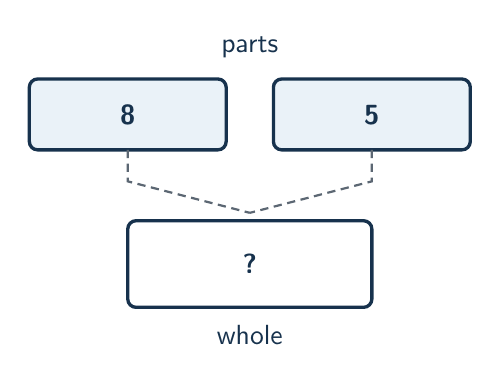
\begin{tikzpicture}[x=1cm,y=1cm]
  \node[qra small label] at (0,2.45) {parts};
  \draw[qra axis, rounded corners=3pt, fill=qraPale] (-2.8,1.15) rectangle (-0.3,2.05);
  \draw[qra axis, rounded corners=3pt, fill=qraPale] (0.3,1.15) rectangle (2.8,2.05);
  \node[qra label] at (-1.55,1.6) {8};
  \node[qra label] at (1.55,1.6) {5};
  \draw[qra guide] (-1.55,1.15) -- (-1.55,0.75) -- (0,0.35);
  \draw[qra guide] (1.55,1.15) -- (1.55,0.75) -- (0,0.35);
  \draw[qra axis, rounded corners=3pt, fill=white] (-1.55,-0.85) rectangle (1.55,0.25);
  \node[qra label] at (0,-0.3) {?};
  \node[qra small label] at (0,-1.2) {whole};
\end{tikzpicture}
\end{document}
